\documentclass[12pt,twocolumn,letterpaper]{article}
\usepackage{epsfig}
\usepackage{amsmath}
\usepackage{amssymb}
\usepackage{graphicx} %package to manage images
\graphicspath{ {images/} }
%%\renewcommand{\baselinestretch}{2}
\usepackage[breaklinks=true,bookmarks=false]{hyperref}
\usepackage{listings} %Package to include

\usepackage{color} %use color
\definecolor{mygreen}{rgb}{0,0.6,0}
\definecolor{mygray}{rgb}{0.5,0.5,0.5}
\definecolor{mymauve}{rgb}{0.58,0,0.82}
 
%Customize a bit the look
\lstset{ %
 backgroundcolor=\color{white}, % choose the background color; you must add \usepackage{color} or \usepackage{xcolor}
 basicstyle=\footnotesize, % the size of the fonts that are used for the code
 breakatwhitespace=false, % sets if automatic breaks should only happen at whitespace
 breaklines=true, % sets automatic line breaking
 captionpos=b, % sets the caption-position to bottom
 commentstyle=\color{mygreen}, % comment style
 deletekeywords={...}, % if you want to delete keywords from the given language
 escapeinside={\%*}{*)}, % if you want to add LaTeX within your code
 extendedchars=true, % lets you use non-ASCII characters; for 8-bits encodings only, does not work with UTF-8
 frame=single, % adds a frame around the code
 keepspaces=true, % keeps spaces in text, useful for keeping indentation of code (possibly needs columns=flexible)
 keywordstyle=\color{blue}, % keyword style
% language=Octave, % the language of the code
 morekeywords={*,...}, % if you want to add more keywords to the set
 numbers=left, % where to put the line-numbers; possible values are (none, left, right)
 numbersep=5pt, % how far the line-numbers are from the code
 numberstyle=\tiny\color{mygray}, % the style that is used for the line-numbers
 rulecolor=\color{black}, % if not set, the frame-color may be changed on line-breaks within not-black text (e.g. comments (green here))
 showspaces=false, % show spaces everywhere adding particular underscores; it overrides 'showstringspaces'
 showstringspaces=false, % underline spaces within strings only
 showtabs=false, % show tabs within strings adding particular underscores
 stepnumber=1, % the step between two line-numbers. If it's 1, each line will be numbered
 stringstyle=\color{mymauve}, % string literal style
 tabsize=2, % sets default tabsize to 2 spaces
 title=\lstname % show the filename of files included with \lstinputlisting; also try caption instead of title
}



\def\cvprPaperID{*} % ** Enter the CVPR Paper ID here
\def\httilde{\mbox{\tt\raisebox{-.5ex}{\symbol{126}}}}

\setcounter{page}{1}

\begin{document}
\title{Organizador de fotos}

\author{Juan de Dios Mart\'inez \\
Instituto Tecnol\'ogico de Costa Rica\\
2016206482\\
\and
Nicol\'as Feoli Chac\'on\\
Instituto Tecnol\'ogico de Costa Rica\\
2016\\
\and
Melisa Cordero Arias\\
Instituto Tecnol\'ogico de Costa Rica\\
2016126133\\
}

\maketitle

\begin{abstract}
Este docummento presenta el an\'alisis de ciertos algoritmos utilizados para el Local Sensitive Hashing (LSH), Local Binary Patterns (LBP) y Pixeles y para lograr llegar a un n\'umero hash y con esto lograr ordenar o clasificar la imagen dependiendo de su similitud al resto de im\'agenes.

\end{abstract}
\section{Introducci\'on}
Esta aplicacion fue dise\~nada con el fin de facilitarle a las personas el hecho de tener que organizar sus fotos cada vez que desean ordenar su tel\'efono. Este app al seleccionarse una foto desde la c\'amara o la galer\'ia, le hace posible al usuario organizarla en 2 versiones, por medio de sus pixeles, o por medio del conocido algoritmo LBP.
Entre estas 2 versiones, es preferible y m\'as \'optimo el LBP ya que su funcionamiento es realmente muy cercano a lo deseado, organizando fotos que son similares y distribuyendo las que no, por otro lado, el algoritmo que utiliza los pixeles tiene un funcionamiento bueno, pero no es el mejor.
Ambos algoritmos utilizan un m\'etodo de Local Sensitive Hashing(LSH), el que se encarga de maximizar las colisiones entre im\'agenes y con ello saber que tan similares son en realidad.

\section{Pixeles}
\subsection{Descripci\'on}
Este metodo de ubicaci\'on de imagenes segun su similitud es uno de los mas simples, por el hecho de que es sencillo de programar y no es tan necesario que sea preciso o exacto.
Para el desarrollo de este algoritmo es necesario tener el m\'etodo que realice el producto punto, y $K$ planos aleatorios constantes para todas las im\'agenes para poder llegar a un resultado mas preciso gracias al algoritmo de LSH.
Al tener la imagen se utiliza un metodo para poder obtener un vector con los pixeles empaquetados de la imagen, para luego realizar el producto punto entre ese vector y el vector $V_1$, luego entre el y $V_2$ hasta realizarlo con $V_k$ y con esto obtener el numero hash de $K$ digitos. Luego se pregunta si el hash ya existe para incluir esta imagen en el bucket correspondiente y si no este se crea.
\\
\begin{lstlisting}[language=Java]

public void pixeles(Bitmap bitmap){
        System.out.println(bitmap);

        bitmap.getPixels(vectorImagen,0,256,0,0,256,256);
        for(int i=0;i<65536;i++){
            vectorImagen[i] = Math.abs(vectorImagen[i]%256);
        }
        //AIUDA
        long hash = productoPunto(vectorImagen, "pixels");
        Bucket b = sing.getBucketPix(hash);
        if(b==null){
            b = new Bucket(Long.toString(hash),hash);
            sing.insertarBucketPix(b);
        }
        b.agregarImagen(bitmap);
    }
}

	\end{lstlisting}

\subsection{Analisis O grande}
El algoritmo de analisis de las im\'agenes por pixeles tiene una $O$ grande de $O(65536*m)$, pues se ejecuta el algoritmo LSH directamente al vector de la imagen, comparando cada pixel de la imagen con cada pixel de cada hiperplano. En este caso, $m$ es el n\'umero de hiperplanos con el que se est\'a trabajando en el momento. 
\section{LBP}
\subsection{Descripci\'on}
El algoritmo LBP se basa en la generaci\'on de un histograma que permite comparar la frecuencia con que ciertos patrones aparecen en un vector. Para ello se compara cada coeficiente del vector con sus vecinos, si el coeficiente que se esta analizando es mayor que el vecino, se coloca un $0$ en la posici\'on correspondiente del hash temporal en caso contrario se coloca un $1$. Luego se le sumar\'a $1$ a la posici\'on [hash] del histograma. Esto se realiza para cada entrada del vector.

\begin{lstlisting}[language=Java]

    public void LBP(Bitmap bitmap){
        int[] histograma = new int[256];
        for(int i=0; i<256; i++) histograma[i] = 0;
        System.out.println(bitmap);
        bitmap.getPixels(vectorImagen,0,256,0,0,256,256);

        for(int i=0;i<65536;i++)
            vectorImagen[i] = Math.abs(vectorImagen[i]%256);
        int hashPixel;
        for(int i=0; i<65536;i++){
            hashPixel = 0;
            if(i<256){//si esta en la fila de arriba
                if(i == 0){
                    //esta en la esquina superior izq
                    if(vectorImagen[i + 1] < vectorImagen[i]) hashPixel += 1; //pixel de derecha
                    hashPixel *= 2; //shift left 1
                    if(vectorImagen[i+257] < vectorImagen[i]) hashPixel += 1; // pixel de esquina inferior derecha
                    hashPixel *= 2;
                    if(vectorImagen[i+256] < vectorImagen[i]) hashPixel += 1; //pixel de abajo
                    hashPixel *= 4; //como esta en la esquina, no se revisan los dos ultimos.
                } else if(i == 255){ //esta en la esquina superior derecha
                    if(vectorImagen[i+256] < vectorImagen[i]) hashPixel += 1; //pixel de abajo
                    hashPixel *= 2; //shift left 1
                    if(vectorImagen[i+255] < vectorImagen[i]) hashPixel += 1;//pixel esquina inf izquierda
                    hashPixel *= 2;
                    if(vectorImagen[i - 1] < vectorImagen[i]) hashPixel += 1; //pixel izquierda
                } else{
                    if(vectorImagen[i + 1] < vectorImagen[i]) hashPixel += 1; //pixel de derecha
                    hashPixel *= 2; //shift left 1
                    if(vectorImagen[i+257] < vectorImagen[i]) hashPixel += 1; // pixel de esquina inferior derecha
                    hashPixel *= 2;
                    if(vectorImagen[i+256] < vectorImagen[i]) hashPixel += 1; //pixel de abajo
                    hashPixel *= 2;
                    if(vectorImagen[i+255] < vectorImagen[i]) hashPixel += 1; //pixel esquina inf izquierda
                    hashPixel *= 2;
                    if(vectorImagen[i - 1] < vectorImagen[i]) hashPixel += 1; //pixel izquierda
                }
            }else if(i >= 65536-256){//si esta en la fila de abajo
                if(i == 0){//esta en la esquina inferior izquierda
                    if(vectorImagen[i-256] < vectorImagen[i]) hashPixel += 1; //pixel arriba
                    hashPixel *= 2;
                    if(vectorImagen[i-257] < vectorImagen[i]) hashPixel += 1; //pixel sup derecha
                    hashPixel *= 2;
                    if(vectorImagen[i + 1] < vectorImagen[i]) hashPixel += 1; //pixel de derecha
                    hashPixel *= 16; //shift left 4, pues no se revisan los ultimos
                }else if(i == 65535){ //esta en la esquina inferior derecha
                    if(vectorImagen[i-257] < vectorImagen[i]) hashPixel += 1; //pixel superior izquierda
                    hashPixel *= 2;
                    if(vectorImagen[i-256] < vectorImagen[i]) hashPixel += 1; //pixel arriba
                    hashPixel *= 64; //shift left 6
                    if(vectorImagen[i - 1] < vectorImagen[i]) hashPixel += 1;//pixel izquierda
                }else{
                    if(vectorImagen[i-257] < vectorImagen[i]) hashPixel += 1;
                    hashPixel *= 2;
                    if(vectorImagen[i-256] < vectorImagen[i]) hashPixel += 1;
                    hashPixel *= 2;
                    if(vectorImagen[i-255] < vectorImagen[i]) hashPixel += 1;
                    hashPixel *= 2;
                    if(vectorImagen[i + 1] < vectorImagen[i]) hashPixel += 1;
                    hashPixel *= 8; //shift left 3
                    if(vectorImagen[i - 1] < vectorImagen[i]) hashPixel += 1;
                }
            }else{//esta en la carnita de la imagen
                if(i%256 == 0){//si esta en la fila de la izuierda
                    if(vectorImagen[i-256] < vectorImagen[i]) hashPixel += 1; //pixel arriba
                    hashPixel *= 2;
                    if(vectorImagen[i-255] < vectorImagen[i]) hashPixel += 1; // esquina superior derecha
                    hashPixel *= 2;
                    if(vectorImagen[i + 1] < vectorImagen[i]) hashPixel += 1; //pixel derecha
                    hashPixel *= 2;
                    if(vectorImagen[i+257] < vectorImagen[i]) hashPixel += 1; // esquina inf derecha
                    hashPixel *= 2;
                    if(vectorImagen[i+256] < vectorImagen[i]) hashPixel += 1; // esquina superior derecha
                    hashPixel *= 4;//shift left 2
                }else if(i%256 == 255){//Esta en la fila de la derecha
                    if(vectorImagen[i-257] < vectorImagen[i]) hashPixel += 1; //pixel superior izq
                    hashPixel *= 2;
                    if(vectorImagen[i-256] < vectorImagen[i]) hashPixel += 1; //pixel arriba
                    hashPixel *= 16;
                    if(vectorImagen[i+256] < vectorImagen[i]) hashPixel += 1; // pixel abajo
                    hashPixel *= 2;
                    if(vectorImagen[i+255] < vectorImagen[i]) hashPixel += 1; // pixel inf izq
                    hashPixel *= 2;
                    if(vectorImagen[i - 1] < vectorImagen[i]) hashPixel += 1; // pixel izquierda
                }
            }
            histograma[hashPixel] += 1;
        }
        long hash = productoPunto(histograma, "lbp");
        Bucket b = sing.getBucketLBP(hash);
        if(b==null){
            b = new Bucket(Long.toString(hash),hash);
            sing.insertarBucketLBP(b);
        }
        b.agregarImagen(bitmap);
        actualizarListView();
    }


	\end{lstlisting}
	
\subsection{Analisis O grande}
La $O$ grande del algoritmo LBP es de $O(256*m+65536*2)$, puesto que para crear el histograma es necesario recorrer cada pixel de la imagen y calcular el n\'umero hash que se forma con los pixeles vecinos. En este caso $m$ es el numero de hiperplanos con los que se compara el algoritmo al efectuar el LSH. De esta forma se concluye que: a pesar de que la eficiencia formal es linear $O(256*m)$ se debe dejar claro que en cualquier caso siempre se van a efectuar al menos 65536 pasos en el algoritmo.
\section{LSH}
\subsection{Descripci\'on}
La aplicacion utiliza un algoritmo de Local Sensitive Hashing que se encarga de que al recibir una imagen, de formato bitmap, este devuelva un Long con el numero de hash que a este le corresponde.
Para el uso de este algoritmo es necesario el uso de K planos, lo que significa que habran $2^K$ posibilidades de hashes.
El LSH se implementa utilizando el producto punto de los hiperplanos del algoritmo con el del vector que se est\'a categorizando.
El algoritmo es el mismo que se conoce generalmente, y muy sencillo de programar ya que solamente es hacer la sumatoria de la multiplicacion entre todos los valores de cada indice de los vectores.
\subsection{An\'alisis O Grande}
La O grande del algoritmo LSH implementado es $O(n*m)$, donde $m$ es la cantidad de planos con los que se va a clasificar el vector de entrada y $n$ la cantidad de dimensiones del vector que se esta comparando. Por lo tanto, cuando se analiza el histograma de texturas del algoritmo LBP se maneja $n=256$  normalmente, mientras que en el de Pixeles $n=65536$ para imagenes de $256$x$256$

\begin{lstlisting}[language=Java]

	public long productoPunto(int[] array1, String tipo){
        int mull = 1;
        long result=0;
        int contador = 256;
        if(tipo.equals("pixels")) contador = 65536;
        for(int i = 0; i< cantBuckets; i++){
            long dot =0;
            int rand[] = randoms.get(i);
            for(int e=0; e<contador; e++){
                dot += array1[e] * rand[e];
            }
            if(dot%2 == 0)
                result += 1*mull;
            mull*=10;
        }
        return result;
    }

	\end{lstlisting}
	
\section{Experimentos}
Uno de los experimentos fue probar con distintos largos de hash para descubrir si la calidad del programa cambia con respecto a la cantidad de digitos que tenga el mismo. Con ambos algoritmos se hicieron las distintas pruebas cambiando el largo del hash. Para pixels se us\'o 2 y 5 de largo y para LBP se us\'o 2 y 10.
Fotos tomadas con el emulador de Android.

\subsection{\textbf{Pixels:}}

\textbf{Hash de 2 digitos:}

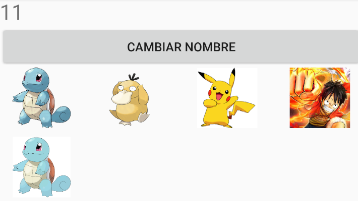
\includegraphics{pix2}

En este hash hay imagenes donde se nota que solo dos de ellas se parecen, pero esto se dice que es por la poca cantidad de diferentes hash que se usan. Se espera que aumentando el numero de planos esto mejore.

\textbf{Hash de 5 digitos:}

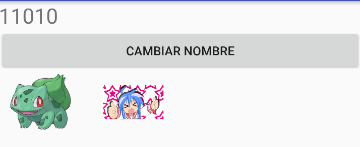
\includegraphics{pix5}

Cuando se utiliza un hash de 5 digitos, lo esperado es que las dos imagenes de squirtle queden en el mismo bucket, y que las otras que no se parecen queden en buckets separados. Pero este no es el caso, misteriosamente los squirtles quedan separados, las unicas imagenes que quedan en un mismo bucket son las que se encuentran anteriormente. Estas imagenes no tienen mucho parecido para nosotros, pero el algoritmo asi las clasifica.

\subsection{\textbf{LBP:}}

\textbf{Hash de 2 digitos:}

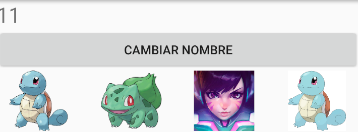
\includegraphics{lbp2}

Utilizando el lbp con 2 de largo en los hash, igual que en pixels los buckets tienen muchas imagenes y la mayor\'ia de ellas no tienen algun parecido. Pero de nuevo esto es por la poca cantidad de posibilidades de obtener un hash diferente

\textbf{Hash de 10 digitos:}

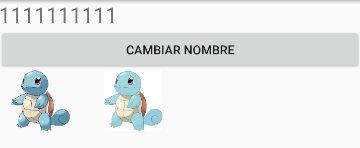
\includegraphics{lbp10}

En este caso si se obtiene el resultado esperado, todas las imagenes se encuentran en buckets separados menos las mostradas anteriormente. Estas se esperaban que quedaran en el mismo bucket desde el inicio porque es la misma imagen solo con algunos variantes en su coloraci\'on.

En ambos algoritmos si se aumentaba el largo del hash todas las imagenes quedaban en buckets separados por lo que decidimos dejarlas en ese n\'umero.

Luego se genera el siguiente grafico para demostrar formalmente el parecido de las imagenes de los buckets, el numero del parecido es un promedio del parecido de las imagenes dentro del bucket.

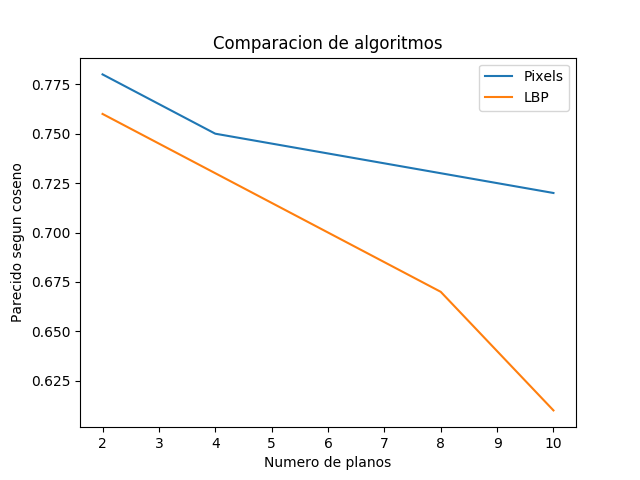
\includegraphics[scale = 0.5]{comparacion}


\section{Conclusi\'on}
En conclusion, podemos observar que este tipo de funciones para una aplicacion no son tan complicadas como lo parecen, puesto que los algortimos existentes para esto tienen una logica similar y sencilla. Y con el uso basico de las mismas podemos crear algo tan funcional como lo es esta aplicacion para repartir imagenes en sus carpetas correspondientes con imagenes parecidas.

\end{document}